\section{Method}
\label{sec:method}

\subsection{FSM design}

The FSM was designed according to the project description and the design procedure given in section \ref{subsec:fsm_theory}. Both a Mealy and a Moore FSM design has been considered. The Mealy state machine resulted in 4 states needed and the Moore machine resulted in 8 states needed, requiring an additional state register and more combinatorial logic. The final design was subsequently chosen to be a Mealy FSM, to minimize the amount of transistors. The state diagram derived from the text description is shown in figure~\ref{fig:fsm_diagram}. To be able to hold four different states, one pause state and three different run states, the FSM needs a 2-bit register, with at least a reset function. 

\begin{figure}[H]
    \centering
    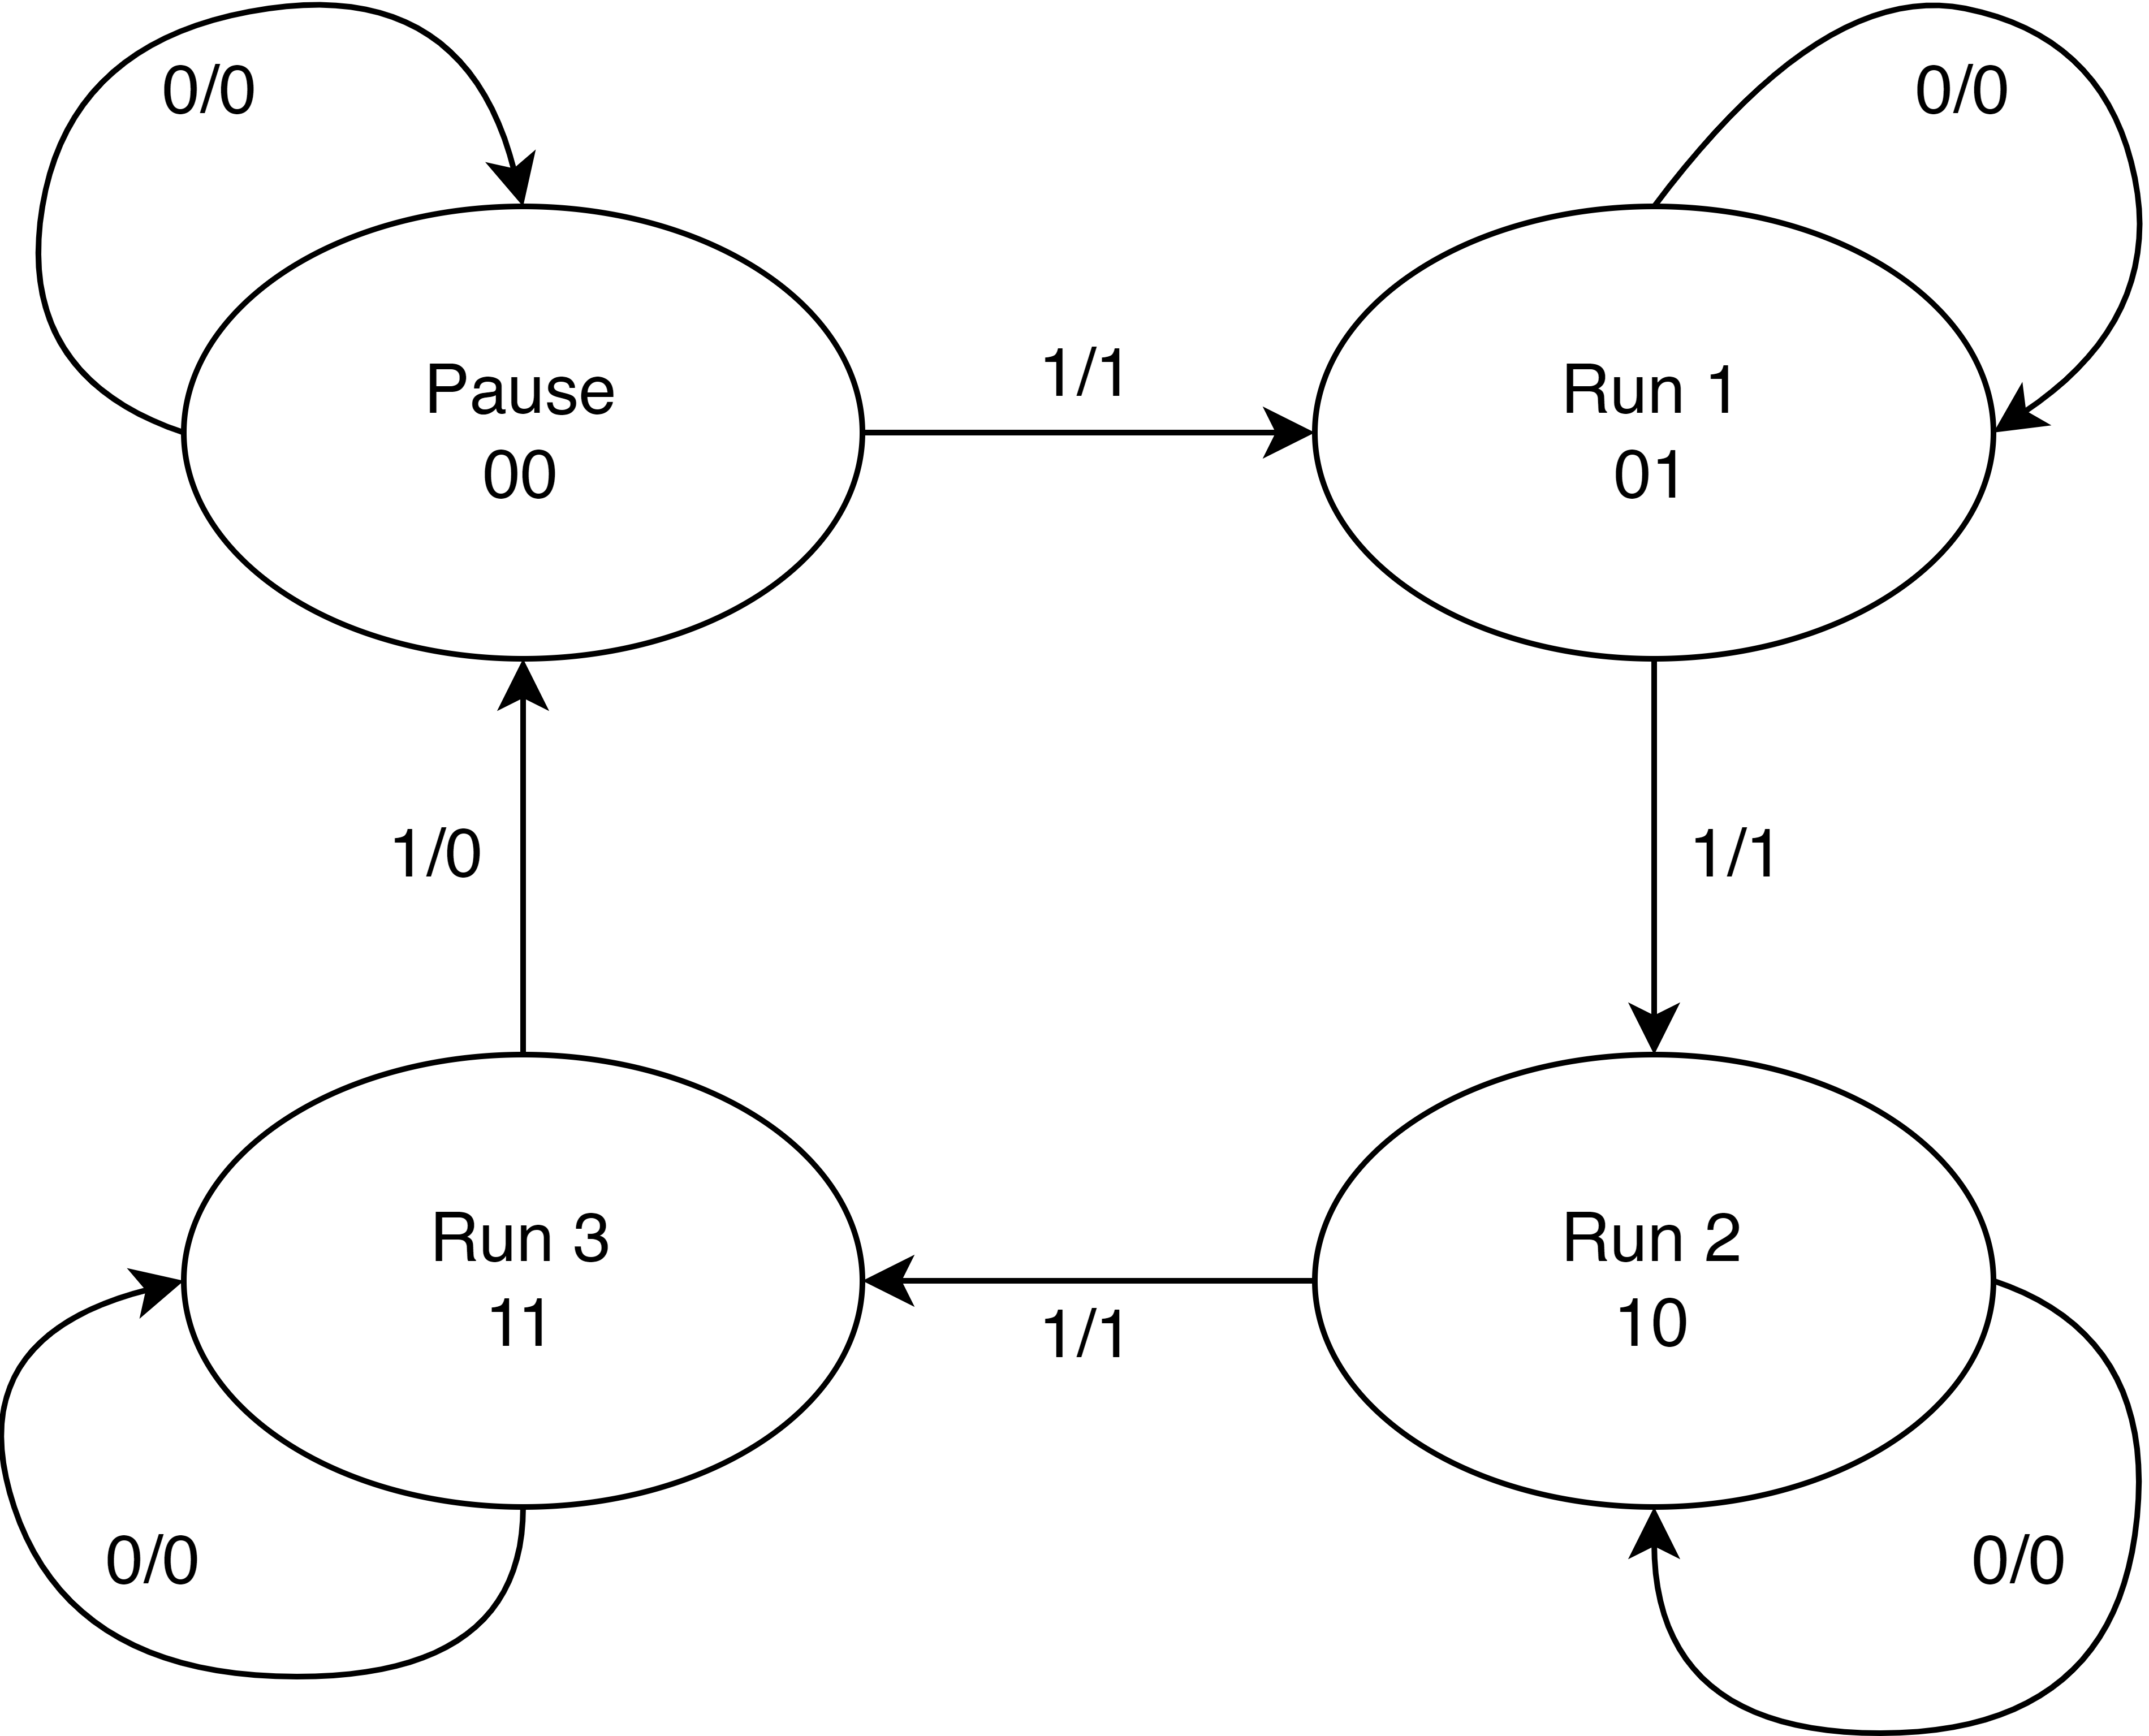
\includegraphics[width=0.8\textwidth]{Figures/FSM-diagram.png}
    \caption{FSM state diagram}
    \label{fig:fsm_diagram}
\end{figure}

Three input signals are given by the project description~\cite{project_description}, Reset, CLK and Run. The CLK-signal
will only be used to time the sequential logic in the FSM and passed on to the MAC unit without
further modification. The CLK signal is therefore not considered an input-signal here in the sense that is not used in the next-state or output-logic in the FSM. The reset signal $I_1$ is only used to reset the state register to the pause-state ''00'' and passed on to the MAC unit as $CTRL_1$ without further modification. The combinatorial part of the FSM is here only dependent on the current state ($C_1$ and $C_0$) and the Run input signal $I_0$. The outputs of the FSM are the next state signals $N_1$ and $N_0$, and the Reset and Run control signals $CTRL_1$ and $CTRL_0$. From the state diagram, we can write the state table~\ref{tab:state_table}. Note that $CTRL_1$ only is dependent on $I_1$ and that this does not require combinatorial logic.

\begin{table}[H]
\caption{State table for the FSM}
\label{tab:state_table}
\centering
\begin{tabular}{|l|l|l|l|l|l||l|l|}
\hline
\rowcolor[HTML]{C0C0C0} 
$C_1$ & $C_0$ & $I_0$ & $N_1$ & $N_0$ & $CTRL_0$ & $I_1$ & $CTRL_1$\\
\hline
0  & 0  & 0  & 0   & 0   & 0 & 1 & 1\\ 
\hline
0  & 0  & 1  & 0   & 1   & 1 & 0 & 0\\ 
\hline
0  & 1  & 0  & 0   & 1   & 0 \\ 
\hline
0  & 1  & 1  & 1   & 0   & 1 \\ 
\hline
1  & 0  & 0  & 1   & 0   & 0 \\ 
\hline
1  & 0  & 1  & 1   & 1   & 1 \\ 
\hline
1  & 1  & 0  & 1   & 1   & 0 \\ 
\hline
1  & 1  & 1  & 0   & 0   & 0 \\ 
\hline

\end{tabular}
\end{table}

\noindent
The logic expression for the outputs of the combinatorial logic can be written down and simplified to equation \ref{eq:comb_eq_1}, \ref{eq:comb_eq_2} and \ref{eq:comb_eq_3}.

\begin{equation}
\label{eq:comb_eq_1}
    CTRL_0 = I_0\cdot(\overline{C_1 \cdot C_0})
\end{equation}

\begin{equation}
\label{eq:comb_eq_2}
    N_0 = C_0 \oplus I_0
\end{equation}

\begin{equation}
\label{eq:comb_eq_3}
    N_1 = C_1 \oplus (C_0 \cdot I_0)
\end{equation}

From the boolean equations, we can draw up the logic diagram shown in figure~\ref{fig:fsm_logic_diagram}.

\begin{figure}[H]
    \centering
    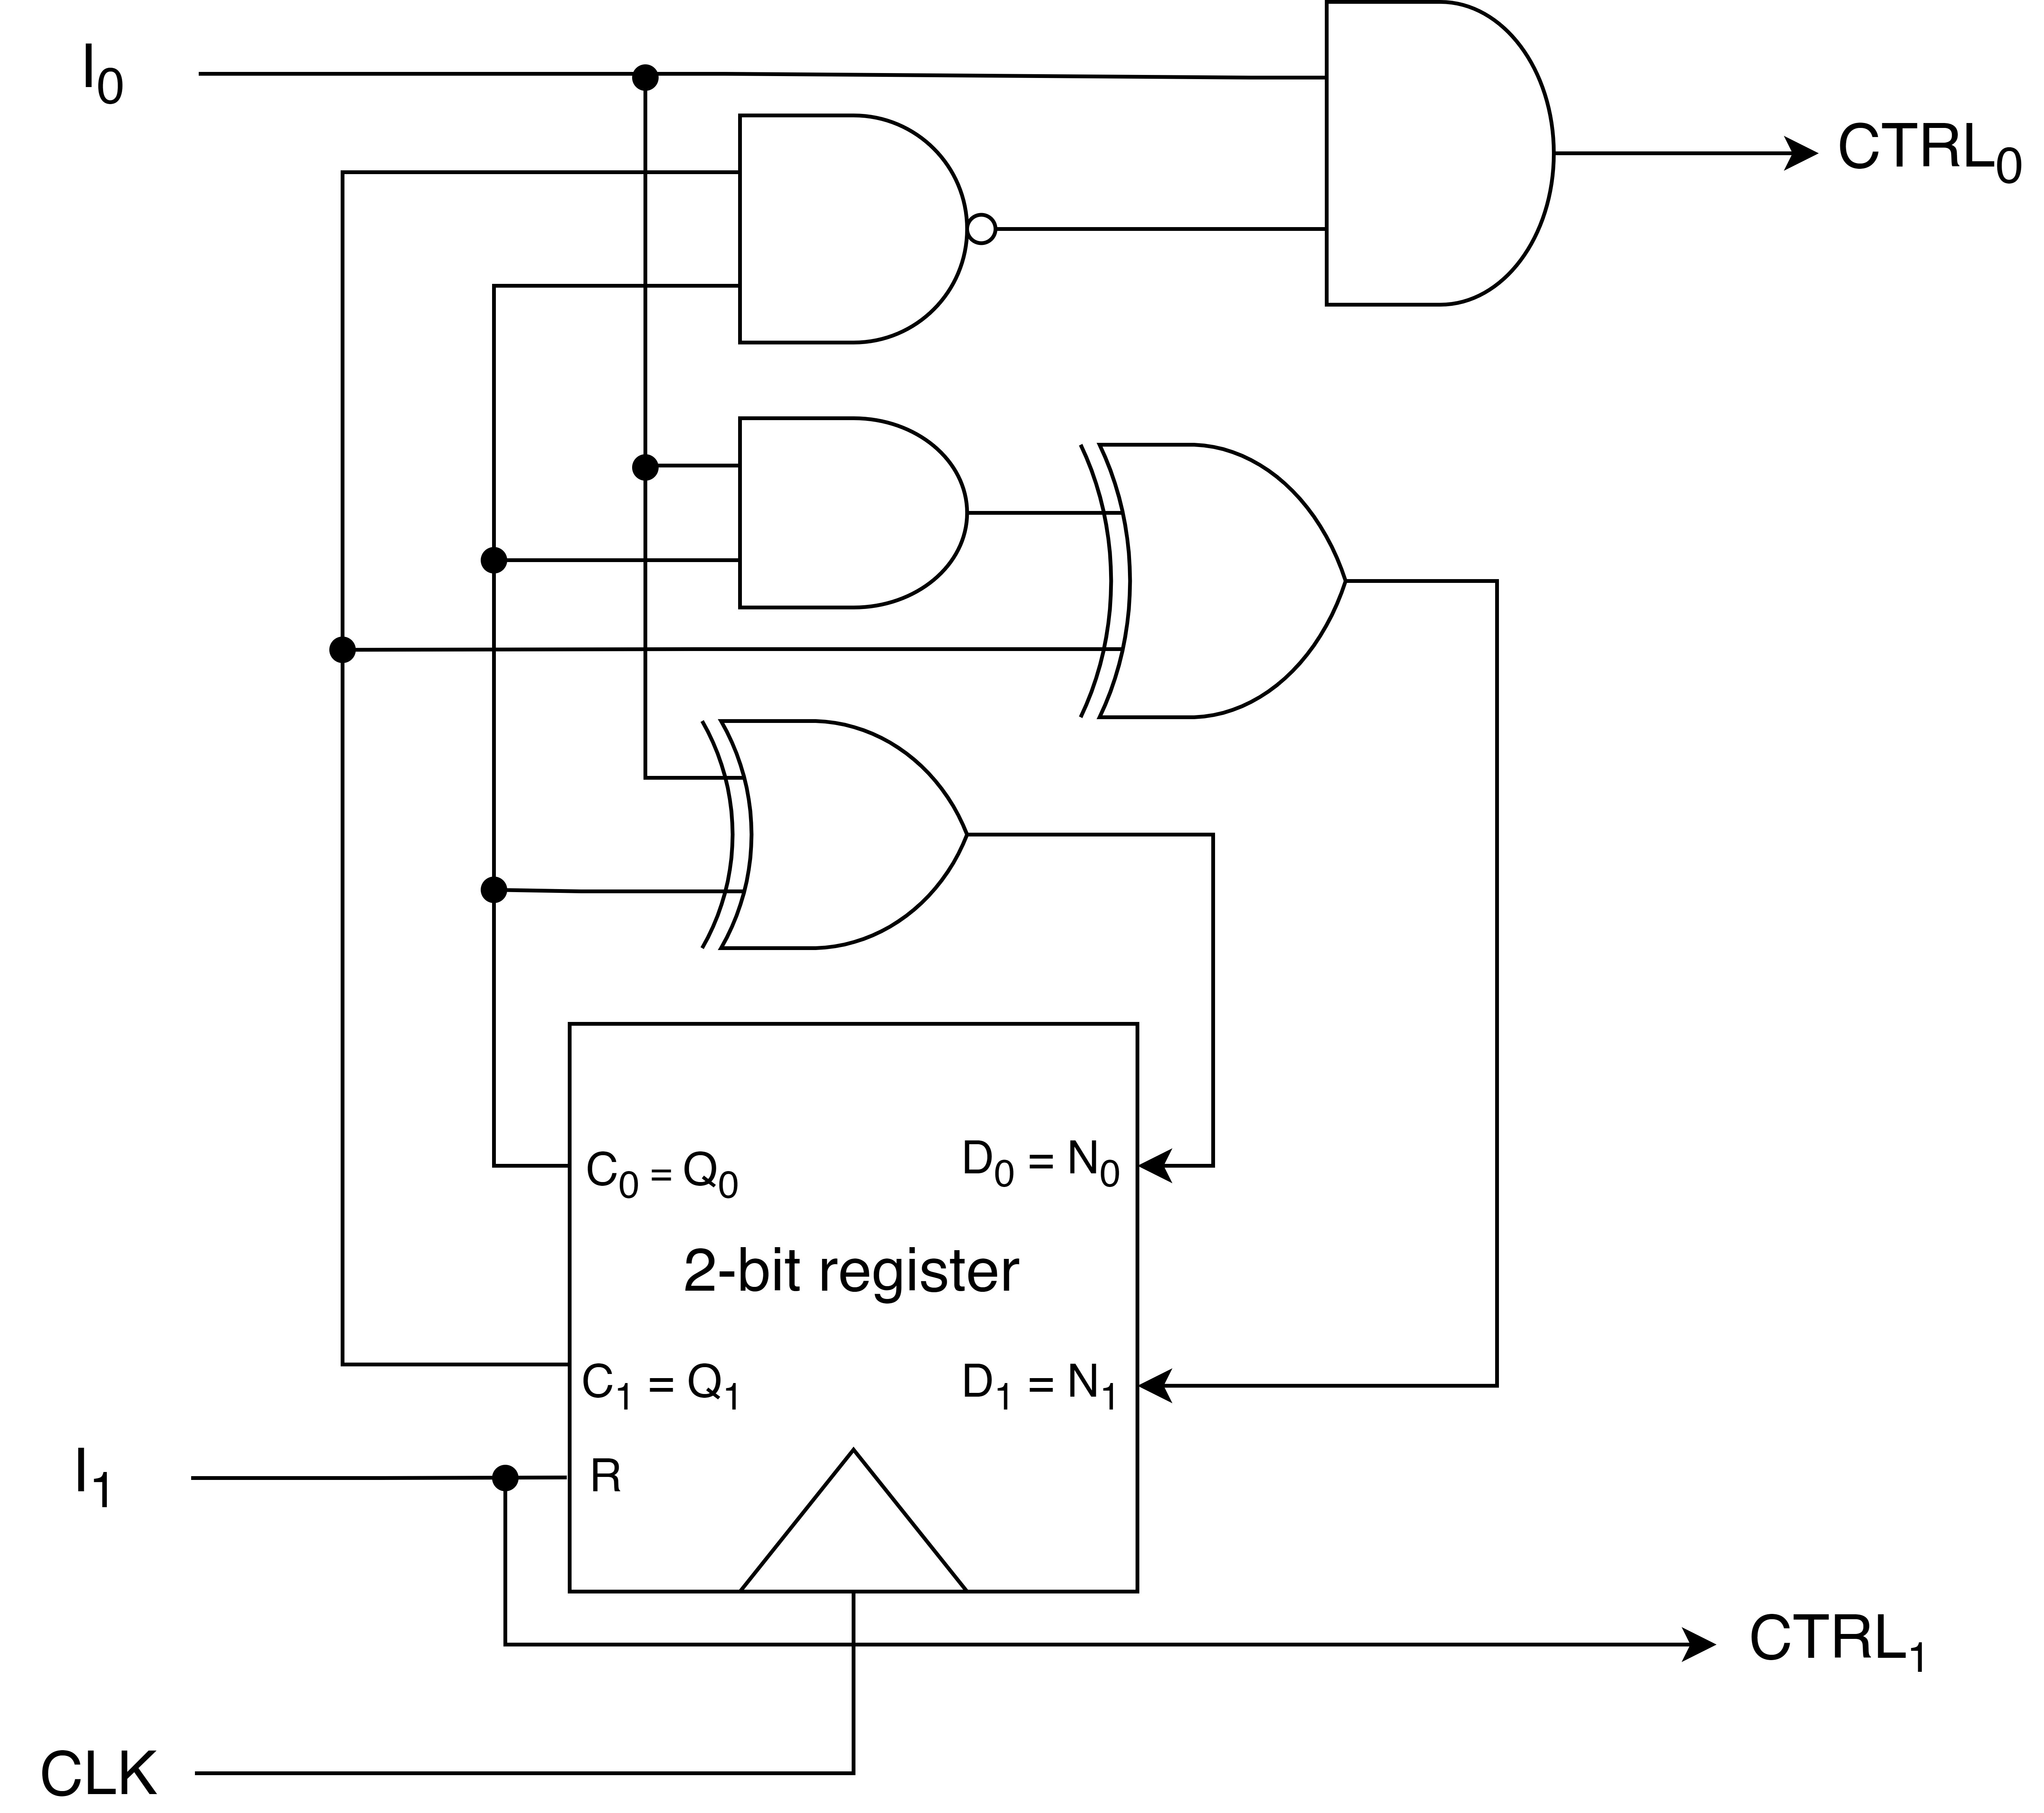
\includegraphics[width=0.6\textwidth]{Figures/logic diagram.png}
    \caption{FSM logic diagram}
    \label{fig:fsm_logic_diagram}
\end{figure}

\noindent
The register used in this circuit is of the same design as the register described in section~\ref{subsubsec:accumulator}.

\subsection{MAC design}
\label{subsec:circuitDesign}

In this section we will look on how to implement the different subsystems of the MAC unit. The designs are shown at a logic gate level as that is used for both the AIMSpice and Verilog implementation. 

\subsubsection{Multiplier} 

A 2-bit multiplier could be designed like shown in figure \ref{fig:multiplier}.

\begin{figure}[H]
    \centering
    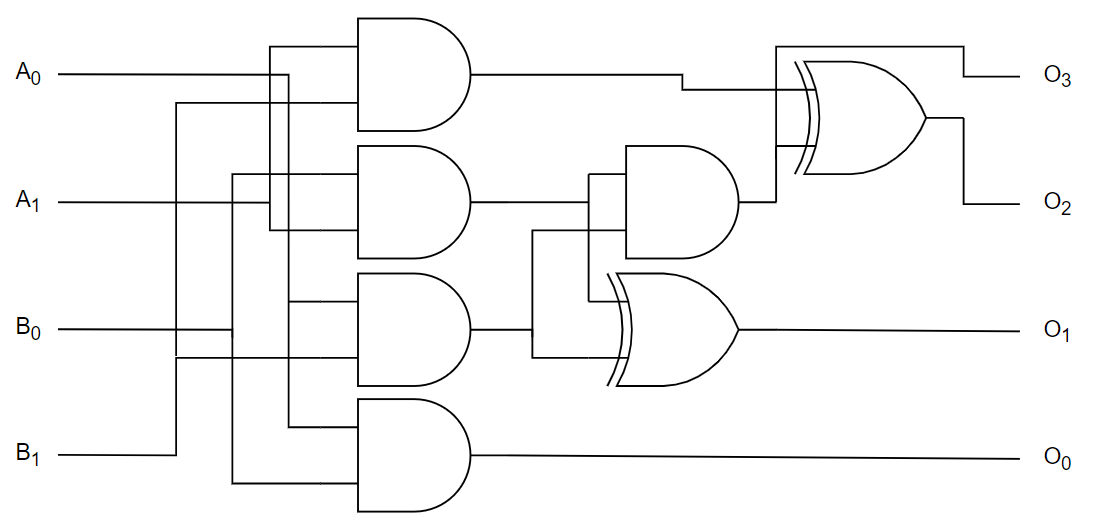
\includegraphics[width=0.8\textwidth]{Figures/multiplier.png}
    \caption{Possible design of multiplier}
    \label{fig:multiplier}
\end{figure}

\subsubsection{Adder}
The circuit for the half and full adder is shown in figure \ref{fig:halfadder} and \ref{fig:fulladder}.

\begin{figure}[H]
\begin{minipage}{0.4\textwidth}
    \centering
    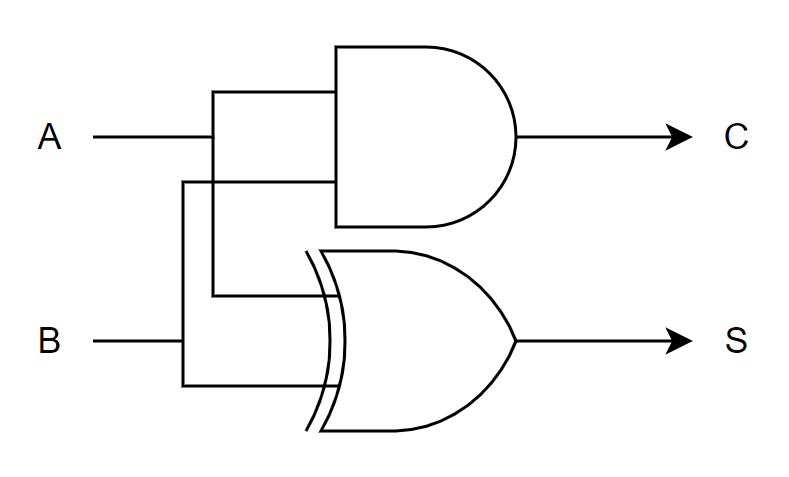
\includegraphics[width=\linewidth]{Figures/halfadder.png}
    \caption{Half adder}
    \label{fig:halfadder}
\end{minipage}
\begin{minipage}{0.6\textwidth}
    \centering
    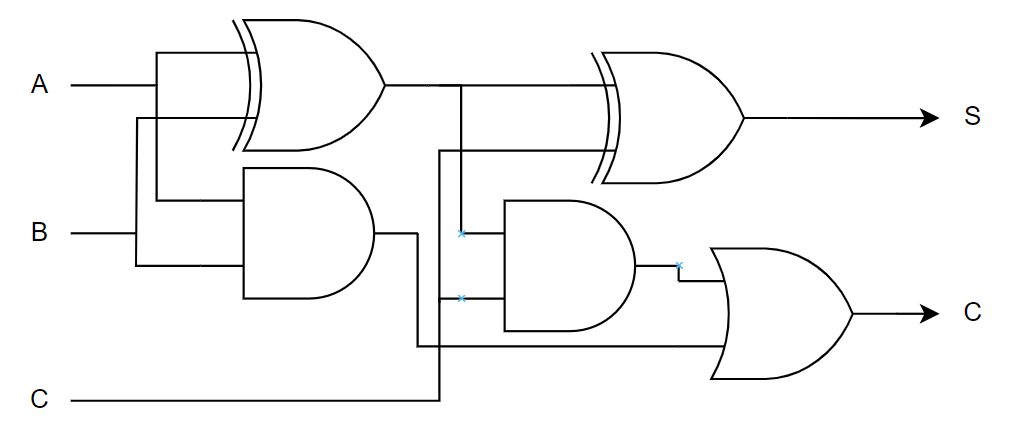
\includegraphics[width=\linewidth]{Figures/fulladder.png}
    \caption{Full adder}
    \label{fig:fulladder}
\end{minipage}
\end{figure}


\subsubsection{Accumulator}
\label{subsubsec:accumulator}
The accumulator is an 8-bit register with some control signals, that is received from the Final State Machine (FSM). As shown in figure \ref{fig:8bitregister}, the accumulator consists of a D-Flip-Flop and a control circuit. These are implemented as shown in figure \ref{fig:dflipflop} and \ref{fig:setreset} respectfully.

\begin{figure}[H]
    \centering
    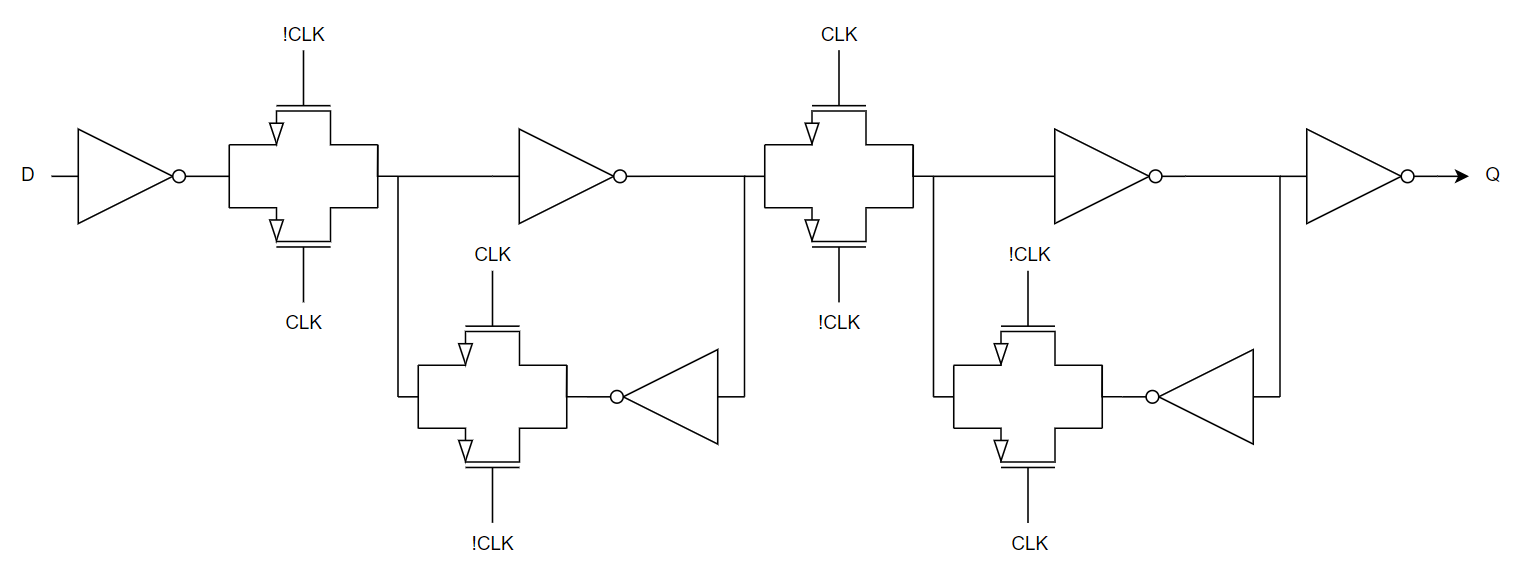
\includegraphics[width=\textwidth]{Figures/D_Flip_Flop.png}
    \caption{D-flip flop}
    \label{fig:dflipflop}
\end{figure}

\begin{figure}[H]
    \centering
    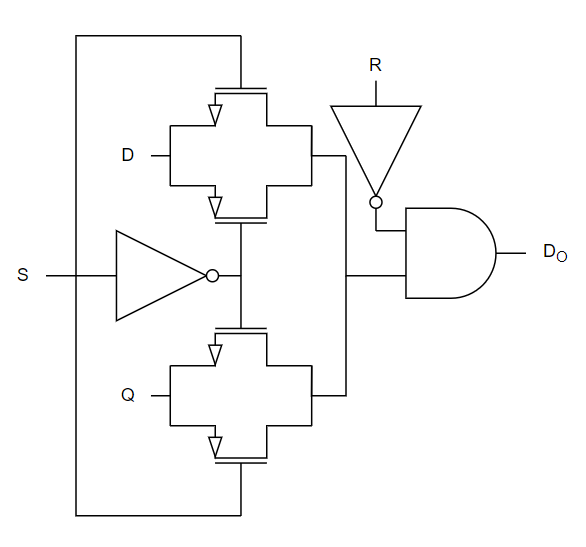
\includegraphics[width=0.4\textwidth]{Figures/setReset.png}
    \caption{Circuit for controlling register}
    \label{fig:setreset}
\end{figure}



\subsection{AimSpice}
In the AimSpice related part of the assignment, a 1 bit register will be implemented using the designs shown in section \ref{subsec:circuitDesign}. 

To implement the register in AimSpice, different logic gates are made using transistors. The different logic gates used in the 1-bit register are NOT-, AND- and transmission gates. This is shown in figure \ref{fig:dflipflop} and \ref{fig:setreset}.

\begin{figure}[H]
\begin{minipage}{0.5\textwidth}
    \centering
    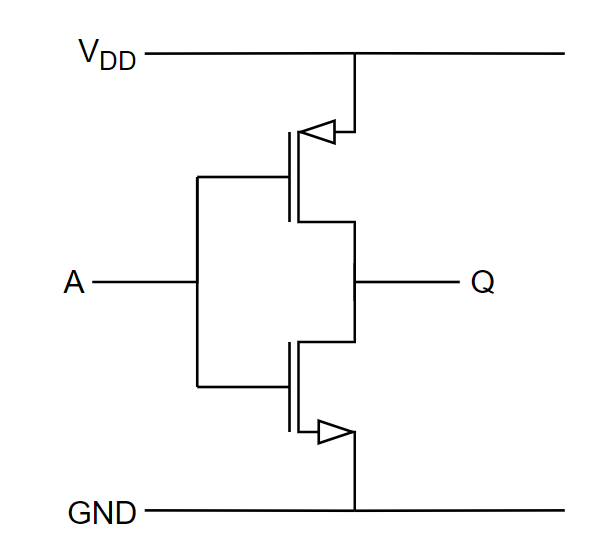
\includegraphics[width=\linewidth]{Figures/Not gate.png}
    \caption{NOT gate using MOSFET}
    \label{fig:NOT}
\end{minipage}
\begin{minipage}{0.5\textwidth}
    \centering
    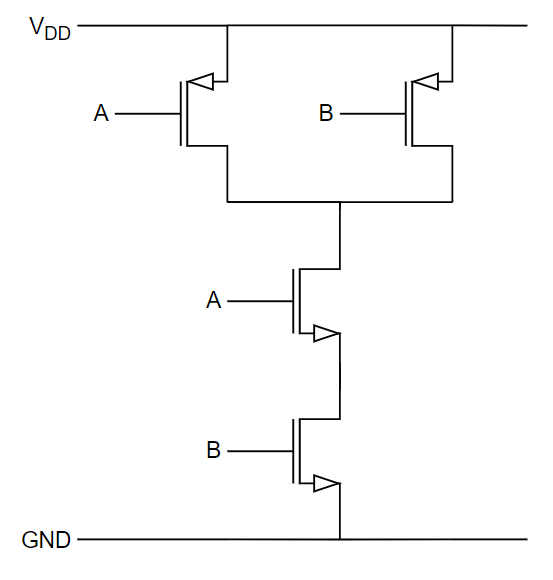
\includegraphics[width=\linewidth]{Figures/Nand Gate.png}
    \caption{NAND gate using MOSFET}
    \label{fig:NAND}
\end{minipage}
\end{figure}

The AND gate is made by connecting a NAND and NOT in series, as shown in figure \ref{fig:AND}.
\begin{figure}[H]
    \centering
    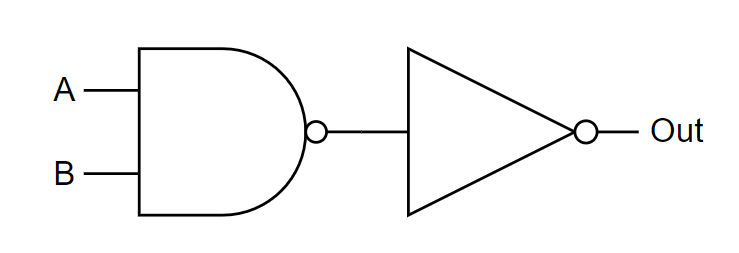
\includegraphics[width=0.4\linewidth]{Figures/And gate.png}
    \caption{AND gate}
    \label{fig:AND}
\end{figure}

\subsubsection{Static CMOS}

\subsection{Verilog}


\subsubsection{Finite State Machine}
\label{subsec:fsm_verilog}

The FSM is implemented and its functionality is verified using the hardware desctriptive language verilog. To simplify the implementation, the register is written as a separate module in listing x. The code for implementing the FSM in verilog is given in listing~\ref{verilog_fsm} in the appendix.

To test the functionality, a separate testbench-module is made in verilog. The FSM is run through a series of different possible inputs. The output timing diagram is subsequently analyzed to verify that the FSM has the correct output based on the input.




In this section you should explain what you have done, and how you have done it. The explanations should have enough detail to make a reproduction possible (i.e. it should be possible to do exactly what you have done, and receive the same results, only by doing what you write in this section).


It might be relevant to refer back to a part of theory, as explained in \autoref{subsec:theory_aSubsection}, to explain the design choices you made.

\subsection{Must include}
The method section MUST INCLUDE:
\begin{itemize}
    \item One or more illustrations showing your circuit. As a minimum you must include one figure of the circuit at the logic gate level, and one of what you implemented at transistor level in AIMSpice.
    \item Figure showing the state diagram for your final state machine (FSM).
    \item Explanations of design choices you made when creating the circuit.
    \item Explanations of the simulations you did (not the results, just how they were done).
\end{itemize}